%% Do not edit unless you really know what you are doing.
\documentclass[french,english,12pt]{exam}

\printanswers

\usepackage{../../latex/macro_mealor}
\usepackage[utf8]{inputenc}
\usepackage[T1]{fontenc} % accents codés dans la fonte
%\usepackage{layout}
\usepackage{a4wide}
%\usepackage[french]{babel}
\usepackage{hyperref}

\usepackage{graphicx}
\usepackage{caption}

\usepackage{newpxtext,newpxmath}
\usepackage{siunitx}

%\setlength{\hoffset}{0pt}
%\setlength{\oddsidemargin}{-1cm}   % Marge gauche sur pages impaires
%\setlength{\evensidemargin}{-1cm}   % Marge gauche sur pages paires
%\setlength{\marginparwidth}{0cm}   % Largeur de note dans la marge
%\setlength{\textwidth}{16cm}   % Largeur de la zone de texte (17cm)
\setlength{\voffset}{0pt}   % Bon pour DOS
\setlength{\marginparsep}{0pt}   % Séparation de la marge
\setlength{\topmargin}{0cm}   % Pas de marge en haut
\setlength{\headheight}{0cm}   % Haut de page
\setlength{\headsep}{0cm}   % Entre le haut de page et le texte
%\setlength{\footskip}{1cm}   % Bas de page + séparation
%\setlength{\textheight}{25.5cm}   % Hauteur de la zone de texte (25cm)

\usepackage{indentfirst}


\newcommand{\classurl}{\url{1}}
% #1 numéro de la feuille
% #2 titre de la feuille
\newcommand{\titre}[3] {%\textit{
  \begin{center}\textbf{\textsc{MEALOR II}}\\ \textit{Mécanique de l'endommagement et approche locale de la rupture}%\let\thefootnote\relax\footnotetext{\classurl} 
  \end{center}
 
  \noindent TD n\textdegree #1 \hfill  August 2023\\[-0.3cm]
  \rule{\linewidth}{.3mm}
  \vspace*{0.5pt}
  \begin{center}
    {
      \Large \bfseries { #2}
    }\\
    \vspace*{0.5cm}
	\large #3
    \vspace*{0.5cm}
  \end{center}
}

\usepackage{xcolor}
\definecolor{Blue}{RGB}{0,68,170}
\SolutionEmphasis{\normalfont\color{Blue}}
\DeclareCaptionFont{blue}{\color{Blue}}

\newenvironment{objectifs}
    {\itshape\underline{Objectifs:}\begin{itemize}
    }
    { \itshape
    \end{itemize}
    }
    
\newcounter{Rfig}
\newenvironment{R_figure}
   {\begin{minipage}{\linewidth}\begin{center}\vspace{0.5mm}\stepcounter{Rfig}\addtocounter{figure}{-1}\renewcommand\thefigure{R-\arabic{Rfig}}
   \captionsetup{font=blue}}
   {\end{center}\vspace{0.5mm}\end{minipage}}
   
    
\newcounter{Rtab}
\newenvironment{R_table}
   {\begin{minipage}{\linewidth}\begin{center}\vspace{0.5mm}\stepcounter{Rtab}\addtocounter{table}{-1}\renewcommand\thetable{R-\arabic{Rtab}}
   \captionsetup{font=blue}
}
   {\end{center}\vspace{0.5mm}\end{minipage}}
   
      
\graphicspath{{./pic/}}
\usepackage{subcaption}
\begin{document}
\thispagestyle{empty}
\titre{2}{Analyse de la ruine d'une structure}{Jérémy Bleyer, Véronique Lazarus}
%\maketitle
\begin{objectifs}
\item Manipuler les concepts de concentration et singularité de contraintes
\item Analyser la ruine d'une structure industrielle
\item Estimer la taille d'un défaut critique et la propagation d'un défaut initial par fatigue
\end{objectifs}

\begin{figure}[ht]
\begin{center}
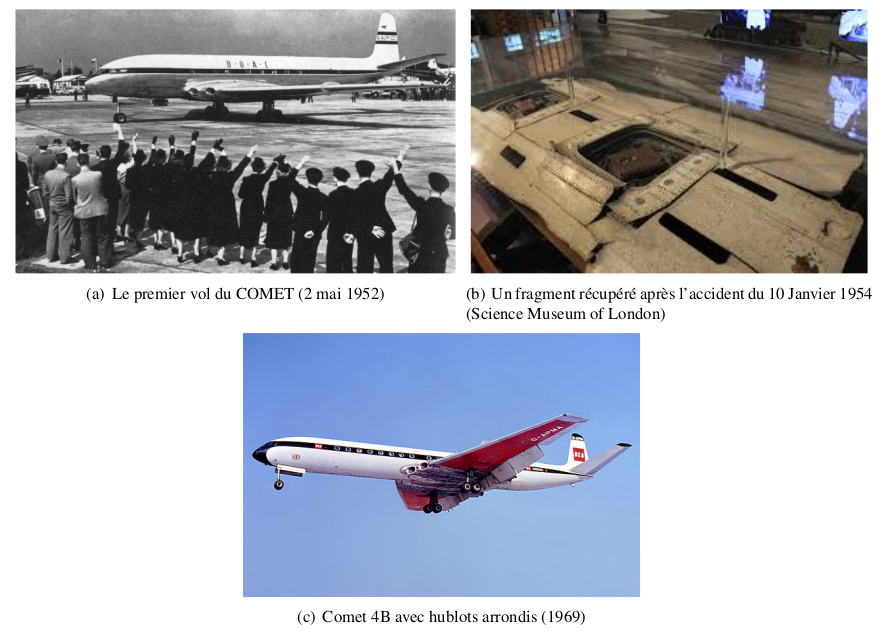
\includegraphics[width=\textwidth]{comet}
\end{center}
\caption{L’évolution du COMET, commercialisé jusque dans les années 80-90}\label{fig:comet}
\end{figure}

\section*{Contexte}

En mai 1952, les Britanniques ont lancé le premier avion de ligne à réaction, le COMET de la société De Havilland (Figure \ref{fig:comet}). Cet avion pouvait voler à 750 km/h sur une distance de 4000 km en transportant 36 passagers. Cependant, l'utilisation d'alliages d'aluminium, mal connus à l'époque, et l'augmentation de l'altitude de vol ont entraîné des évolutions imprévues des structures en raison d'un phénomène de fatigue qui n'avait pas été pris en compte lors de la conception.

Deux ans après son lancement, le 10 janvier et le 8 avril 1954, deux avions COMET se sont écrasés dans des circonstances alors inexpliquées. Les ingénieurs ont constaté que les accidents se sont produits lorsque les avions avaient atteint leur altitude de croisière de 10 000 m, où la différence de pression entre l'intérieur et l'extérieur atteignait son maximum en raison de la pressurisation de la cabine à environ 1 atm. Ils ont soupçonné une défaillance du fuselage.

Des essais au sol ont été réalisés sur une cabine identique, soumise à des pressions internes cycliques, et les ingénieurs ont observé la propagation brutale d'une fissure initiée au niveau d'un hublot. Suite à cette découverte, la forme des hublots a été modifiée et arrondie pour atténuer la concentration des contraintes.

Contrairement à ce que l'on croyait alors, la durée de vie de l'avion était déterminée principalement par le nombre de décollages et d'atterrissages (cycles gonflement-dégonflement de la cabine) et non par le nombre d'heures de vol. L’objectif de ce TD est d’estimer ce nombre de cycles par une analyse mécanique simplifiée d’un fuselage
d’avion comportant des hublots circulaires rivetés, puis de le comparer au nombre effectif d’environ 750 décollages
recensés avant les accidents.

\section*{Données du problème}

\begin{figure}
\begin{center}
\begin{subfigure}[b]{0.49\textwidth}
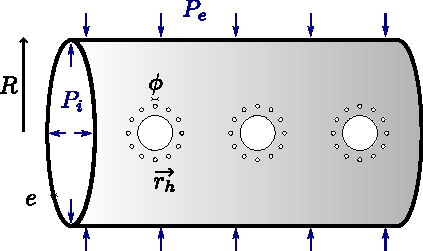
\includegraphics[width=\textwidth]{geometry_simplified}
\caption{Géométrie simplifiée: fuselage, hublots et rivets}\label{fig:geometrie}
\end{subfigure}
\hfill
\begin{subfigure}[b]{0.49\textwidth}\centering
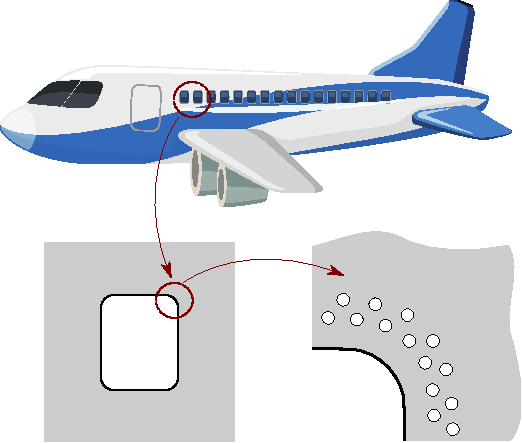
\includegraphics[width=0.8\textwidth]{multiscale}
\caption{Analyse multi-échelles}\label{fig:analyse}
\end{subfigure}
\end{center}
\caption{Modélisation du problème}
\end{figure}

\subsection*{Géométrie}
On modélise le fuselage de l’avion par une enveloppe cylindrique fermée à ses deux extrémités (fig. \ref{fig:geometrie}). Sa
partie courante est de rayon $R = \SI{3}{m}$ et d’épaisseur $e = \SI{2}{mm}$. Le fuselage est percé de hublots circulaires de rayon $r_h = \SI{15}{cm}$. La distance entre les hublots est de l’ordre de \SI{1.5}{m}. Les hublots sont fixés par des rivets placés dans des trous du fuselage, de diamètre $\phi = \SI{5}{mm}$, dont les centres sont à \SI{2}{cm} du bord du trou du hublot. Le bord du trou d’un rivet peut comporter une fissure initiale dont la taille est liée à celle des grains constituant le matériau. Nous supposerons que la fissure peut avoir une longueur initiale $a_0 = \SI{30}{\micro\meter}$ pour cet alliage d'aluminium.

\subsection*{Chargement}
Le chargement à prendre en compte pour l’étude de la propagation des fissures est constitué par les pressions interne
$P_i$ et externe $P_e$. Lorsque l'avion est au sol, les pressions interne et externe sont égales et valent $\SI{10}{kPa}$. La pression $P_i$ est supposée rester constante, alors que $P_e$ varie à chaque décollage de $\SI{10}{kPa}$ au sol, à $\SI{4.8}{kPa}$ à $\SI{10000}{m}$.
Nous noterons $\Delta P = P_i - P_e$ la différence de pression.


\subsection*{Matériau}
Le matériau est un alliage d’aluminium considéré ici dans son domaine élastique linéaire avec un module d’Young
$E = \SI{70}{GPa}$ et un coefficient de Poisson $\nu = 0.3$.


\section{Analyse multi-échelle du problème}

L’analyse du problème comporte deux parties. La première porte sur la détermination du champ de contraintes au
voisinage de l’extrémité de la fissure, car c’est lui qui pilotera son avancée et la ruine catastrophique de la structure.
Elle se fera par une approche multi-échelle simplifiée (cf. fig. \ref{fig:analyse}), analytique, comportant les points suivants:
\begin{itemize}
\item Détermination des contraintes dans le fuselage soumis à des pressions interne et externe;
\item Calcul du champ de contraintes au bord du hublot en considérant celui-ci comme une cavité circulaire dans une
plaque mince soumise à l’infini au champ précédent;
\item Calcul du champ de contraintes au bord du trou de rivet considéré comme une cavité circulaire dans une plaque
mince soumise à l’infini au champ généré autour le hublot.
\item Détermination de la singularité des contraintes en pointe de fissure.
\end{itemize}

La deuxième partie porte sur l’étude de la propagation de la fissure au niveau du trou de rivet sous l’effet des cycles
de pressurisation.

\subsection{Détermination du champ de contraintes au voisinage de la fissure}
\subsubsection{Champ de contraintes dans la partie courante du fuselage}

Nous allons déterminer par le raisonnement dit "du chaudronnier" le tenseur des contraintes $\tenseur{\Sigma}$ dans le fuselage, loin des extrémités et en ignorant la présence des hublots. Le fuselage sera
considéré en première approximation comme un récipient cylindrique de révolution d’axe $\tenseur{e_z}$ fermé par deux calottes (par ex. hémisphériques) aux extrémités.

\begin{questions}
\question En première approximation, $\Sigma_{\theta\theta}$ et $\Sigma_{zz}$ sont pris uniformes dans l’épaisseur du fuselage. Montrer que l’on a $\Sigma_{\theta\theta} = 2 \Sigma_{zz} = (P_i - P_e)R/e$ et que $\Sigma_{rr}$ peut être négligé par rapport aux autres composantes. \textit{On pourra raisonner sur l'équilibre global d'une coupe selon un plan de normale $\tenseur{e_z}$ puis de normale $\tenseur{e_x}$}.
\begin{solution}
Il s'agit du problème classique de l'enveloppe cylindrique sous pression. En écrivant l'équilibre transverse d'une tranche de demi cylindre, on trouve d'abord
$$ 2e \Sigma_{\theta \theta} = 2 R_i P_i - 2 R_e P_e \approx 2 R (P_i - P_e).$$
En écrivant l'équilibre axial d'une des calottes de bout de fuselage, on trouve
$$( \pi R_e^2 - \pi R_i^2) \Sigma_{zz} = P_i \pi R_i^2 -P_e  \pi R_i^2$$
ce qui, pour de faibles épaisseurs, donne
$$2e R  \sigma_{zz} = (P_i-P_e) R^2.$$
Du fait de la grande valeur de $R/e$, la contrainte radiale qui est de l'ordre de $P_i$ peut être négligée par rapport aux deux autres valeurs. 
\end{solution}
\end{questions}

\subsubsection{Analyse du voisinage du bord des hublots}

Pour une analyse approchée simple du champ de contraintes au voisinage des hublots:
\begin{itemize}
\item  nous supposerons que les différents hublots ont peu d’influence les uns sur les autres, car la distance entre
hublot est grande par rapport à leur taille;
\item  nous négligerons l’influence des trous des rivets, car ceux-ci sont de très petite taille par rapport au rayon du
hublot;
\item nous négligerons le rayon de courbure du fuselage (car $r_h\ll R$) et supposerons les hublots inclus dans une
plaque plane soumise à l’infini à un champ de contraintes :
\begin{equation}
\sigma^\infty = \sigma_1 \tenseur{e_X} \otimes \tenseur{e_X} + \sigma_2 \tenseur{e_Y} \otimes \tenseur{e_Y}
\label{eq:plaque-infinie-biaxial}
\end{equation}
avec $\sigma_1 = \Sigma_{zz}$ et $\sigma_2 = \Sigma_{\theta\theta}$ (on note $(\tenseur{e_X} , \tenseur{e_Y}$) les vecteurs du plan correspondant à $(\tenseur{e_z},\tenseur{e_\theta}$) dans la géométrie du cylindre de
révolution).
\item on se placera en situation de contraintes planes, i.e. $\sigma_{zz} = 0$, $\tenseur{\sigma}$ indépendant de $z$ (car $|\Sigma_{rr}| \ll \Sigma_{zz}$).
\end{itemize}

 Le problème de la plaque plane élastique  en contrainte plane, de dimension infinie 
percée d'un trou circulaire de rayon $a$ et soumise à l'infini au champ de 
contrainte $\tenseur{\sigma} ^\infty  =\sigma _\infty
\tenseur{e_X}\otimes \tenseur{e_X}$ admet une solution analytique\footnote{Cette solution s'obtient classiquement par l'usage d'une fonction d'Airy.} qui est donnée en coordonnées cylindriques liées au trou par
\begin{subequations}
\begin{eqnarray}
&& \sigma_{rr} = \frac{\sigma_\infty}{2}\left(1-\frac{a^2}{r^2}\right)+ \frac{\sigma_\infty}{2}\left(1+ \frac{3a^4}{r^4}-\frac{4a^2}{r^2}\right) \cos (2\theta),\\
&& \sigma_{\theta \theta} = \frac{\sigma_\infty}{2}\left(1+\frac{a^2}{r^2}\right)- \frac{\sigma_\infty}{2}\left(1+ \frac{3a^4}{r^4}\right) \cos (2\theta),\\
&& \sigma_{r\theta} = - \frac{\sigma_\infty}{2}\left(1- \frac{3a^4}{r^4}+\frac{2a^2}{r^2}\right) \sin(2\theta), \\
&& \sigma_{rz}= \sigma_{\theta z}= \sigma_{zz} =0.
\end{eqnarray}
\label{eq:solution-traction-uniaxiale}
\end{subequations}

\begin{questions}
\question Vérifier que cette solution satisfait bien les conditions aux limites en bord de trou et à l'infini.  Quel champ de contraintes prédit-elle en bord de trou pour un chargement uniaxial?
\begin{solution}
Bien que ce n'était pas demandé, on pourra faire remarquer que le champ proposé vérifie bien l'équilibre local $\divergence{ \tenseur{\sigma}}=0$. De plus, on trouve en bord de trou $r=a$:
$$\tenseur{\sigma} = \sigma_\infty (1- 2 \cos (2 \theta)) \tenseur {e}_\theta \otimes \tenseur{e}_\theta,$$ 
qui vérifie bien la condition de bord libre $\tenseur{\sigma} \cdot \tenseur{e}_r = 0$.

\`A l'infini, il reste
$$
\tenseur{\sigma} = \frac{\sigma_\infty}{2}( (1 + \cos (2 \theta)) \tenseur{e}_r \otimes \tenseur{e}_r+ (1 - \cos (2 \theta)) \tenseur{e}_\theta \otimes \tenseur{e}_\theta  - \sin (2 \theta) ( \tenseur{e}_r \otimes \tenseur{e}_\theta + \tenseur{e}_\theta \otimes \tenseur{e}_r))
= \sigma_\infty \tenseur{e}_X \otimes \tenseur{e}_X
$$
après développement de $\tenseur{e}_r$ en $\tenseur{e}_r = \tenseur{e}_X \cos \theta + \tenseur{e}_Y \sin \theta$ et  de $\tenseur{e}_\theta$ en $\tenseur{e}_\theta = -\tenseur{e}_X \sin \theta + \tenseur{e}_Y \cos \theta$.

Cette solution équilibre la contrainte axiale à l'infini par une contrainte orthoradiale en bord de trou. On constate que pour $\theta=0,\pi$, on a une compression $\sigma_{\theta\theta}(r=a)=-\sigma_\infty$ tandis qu'en $\theta=\pm\pi/2$, on a une traction $\sigma_{\theta\theta}(r=a)=3\sigma_\infty$, c'est à dire un facteur de concentration de contrainte de 3.
\end{solution}

\question Déterminer le champ solution pour le chargement \eqref{eq:plaque-infinie-biaxial} et analyser l'état de contrainte en bord de hublot.
\begin{solution}
Par superposition, la solution est obtenue en combinant une traction uniaxiale d'intensité $\sigma_1$ selon $\tenseur{e}_X$ ainsi qu'une traction uniaxiale d'intensité $\sigma_2$ selon $\tenseur{e}_Y$.
Pour le chargement selon $\tenseur{e}_X$, la solution correspond à \eqref{eq:solution-traction-uniaxiale} en remplaçant $\sigma_{\infty}$ par $\sigma_1$.

Pour le chargement selon $\tenseur{e}_Y$, la solution est obtenue à partir de \eqref{eq:solution-traction-uniaxiale} en remplaçant $\sigma_{\infty}$ par $\sigma_2$ et $\theta$ par $\pi/2-\theta$, soit:
\begin{eqnarray*}
&& \sigma_{rr} = \frac{\sigma_2}{2}\left(1-\frac{a^2}{r^2}\right)- \frac{\sigma_2}{2}\left(1+ \frac{3a^4}{r^4}-\frac{4a^2}{r^2}\right) \cos (2\theta),\\
&& \sigma_{\theta \theta} = \frac{\sigma_2}{2}\left(1+\frac{a^2}{r^2}\right)+\frac{\sigma_2}{2}\left(1+ \frac{3a^4}{r^4}\right) \cos (2\theta),\\
&& \sigma_{r\theta} = - \frac{\sigma_2}{2}\left(1- \frac{3a^4}{r^4}+\frac{2a^2}{r^2}\right) \sin(2\theta), \\
&& \sigma_{rz}= \sigma_{\theta z}= \sigma_{zz} =0.
\end{eqnarray*}

En bord de hublot, on a alors:
$$\tenseur{\sigma} = \sigma_1 (1- 2 \cos (2 \theta)) + \sigma_2(1+2\cos(2\theta)) \tenseur {e}_\theta \otimes \tenseur{e}_\theta
$$
soit avec $\sigma_1=\Sigma_{zz}=\Delta P R/2e$ et $\sigma_2 = \Sigma_{\theta\theta}=\Delta P R/e$:
$$\tenseur{\sigma} = \Delta P \dfrac{R}{e}\left(\dfrac{3}{2}+ \cos (2 \theta)\right) \tenseur {e}_\theta \otimes \tenseur{e}_\theta
$$
La traction est maximale en $\theta=0$ et vaut $\sigma_\text{hublot} = \dfrac{5}{2}\Delta P \dfrac{R}{e}$. Nous voyons ainsi que
le hublot joue un rôle de concentration de contraintes (avec un facteur 5/2).
\end{solution}
\end{questions}

\subsection{Analyse du voisinage du bord des trous des rivets}
Les trous de rivets ont un diamètre de 5mm. Ils sont placés à 2cm du bord du trou du hublot qui a lui-même un rayon de 15cm. Le trou de rivet le plus sollicité se trouve sur l'axe réel ($\underline{OM}=X\tenseur{e}_X,\;\;X\ge r)$. C'est donc ce trou que nous allons étudier.
 
En première approximation, nous pouvons supposer que ce trou de rivet est suffisamment loin du bord du trou du hublot pour ne pas être influencé par celui-ci. Nous pouvons donc en première approximation considérer la solution d'une plaque infinie percée d'un trou circulaire soumise à l'infini au champ de contrainte $\tenseur{\sigma} ^\infty =\sigma_\text{hublot} \tenseur{e}_Y\otimes 
\tenseur{e}_Y$. 

En se plaçant dans le repère cylindrique associé au rivet, calculer la valeur maximale de la traction orthoradiale $\sigma_{\theta \theta} $ en bord de rivet
$\sigma_\text{rivet} = \max_{\theta} \sigma_{\theta \theta}(a) $. Effectuer l'application numérique.

\begin{solution}
On est ici dans le cas d'une plaque infini à trou circulaire chargée à l'infini par une traction uniaxiale $\sigma_\infty=   \sigma_\text{hublot}$. D'après la solution analytique proposée, la tenseur des contraintes en bord de rivet a pour composante unique
$$
 \sigma_{\theta \theta} =\sigma_\text{hublot}(1+2 \cos 2 \theta)
$$  
qui est maximale en $\theta =0,\pi$, soit perpendiculairement au chargement appliqué, et qui a pour valeur $$\sigma_\text{rivet}= 3 \sigma_\text{hublot} = \dfrac{15}{2} \Delta P \dfrac{R}{e} \approx \SI{585}{MPa}.$$            

Ainsi le trou de rivet joue le rôle d’un second ”concentrateur de contraintes”. Le facteur de concentration de
contraintes est maintenant de 15/2. C’est en ce point particulièrement sollicité de la structure que l’initiation et la
propagation d’une micro-fissure est la plus probable et la plus dangereuse.

Notons également que la valeur numérique trouvée pour la contrainte est relativement élevée et peut potentiellement mettre en défaut l'hypothèse d'une étude dans le régime élastique linéaire.
\end{solution}

\section{Propagation de défaut critique}
Le bord de rivet est donc la région la plus sollicitée de la structure. Nous considérons la présence d'un défaut initialement sous la forme d'une fissure débouchant dans le rivet et de taille $a_0=\SI{30}{\micro\meter}$.
\begin{questions}
\question Quelle est la position et l'orientation de la fissure la plus défavorable pour la ruine de la structure ?
\begin{solution}
Le cas le plus défavorable correspond à une sollicitation de la fissure en mode I pur. Le rivet étant chargé par une traction selon $\tenseur{e}_Y$, le cas le plus défavorable correspond donc à une fissure située en $\theta=0,\pi$ et alignée suivant $\tenseur{e}_X$.
\end{solution}

\question Nous admettrons que pour une fissure de longueur $a$ débouchant au bord d'une plaque rectangulaire et soumise à une traction parallèle
au bord de la plaque d’intensité $\sigma$, le facteur d’intensité des contraintes vaut approximativement
\begin{equation}
K_I = 1.12\sigma\sqrt{\pi a}
\end{equation}
Justifier que ce même facteur d'intensité de contraintes peut-être utilisé pour analyser la singularité de contrainte en pointe de la fissure.
\begin{solution}
Il s'agit de la même situation à la différence du fait que le bord libre est courbe (rivet circulaire) et non pas droit comme dans la plaque rectangulaire. Cependant, le diamètre du rivet vaut $\phi=\SI{5}{mm} \gg a_0$ ce qui fait qu'on peut négliger l'effet du rayon de courbure du bord libre devant la taille de la fissure. On a donc:
$$K_I = 1.12\sigma_\text{rivet}\sqrt{\pi a_0} $$
\end{solution}

\question La ténacité du matériau $K_c$ correspondant au seuil de propagation de fissure vaut $K_c =\SI{40}{MPa.m^{1/2}}$. La fissure de taille $a_0$ peut-elle se propager de manière brutale ? Sinon, quelle serait la taille $a_c$ du défaut critique à considérer conduisant à une rupture brutale du fuselage ?
\begin{solution}
On trouve ici $K_I \approx \SI{6.36}{MPa.m^{1/2}}$, soit $K_I < K_c$. La fissure ne peut donc pas se propager. On notera qu'on suppose implicitement que la propagation, si elle a lieu, est instable. 

La taille maximale du défaut critique à considérer menant à la propagation est donc telle que:
$$
K_c = 1.12\sigma_\text{rivet}\sqrt{\pi a_c} = K_I(a_0)\sqrt{\dfrac{a_c}{a_0}}
$$
soit:
$$a_c = a_0 \left(\dfrac{K_c}{K_I(a_0)}\right)^2 \approx \SI{1.19}{mm}$$

On pourra remarquer qu'un tel défaut est difficilement visible à l'oeil nu.
\end{solution}
\end{questions}

\section{Analyse de la ruine par fatigue}
Sous chargement cyclique, les fissures croissent à chaque cycle de chargement par fatigue. Dans le cas de l'aluminium, l’accroissement de longueur de fissure par cycle (noté $\frac{da}{dN}$) est donné par la loi de Paris:
\begin{equation}
\dfrac{da}{dN}
= \beta(\Delta K)^3
\end{equation}
avec $\beta=3.10^{-28}\,\unit{Pa^{-3}.m^{-1/2}/cycle}$ et où $\Delta K$ désigne l'amplitude de variation du facteur d'intensité de contrainte sur un cycle. 

\begin{questions}
\question Caractériser comment un défaut de taille $a_0$ peut conduire à la ruine de la structure après un certain nombre de vols.
\begin{solution}
\`A chaque décollage de l'avion, la différence de pression lors d'un cycle passe de 0 à $\Delta P$. Cela induit une variation de facteur d'intensité de contrainte $\Delta K(a) =  1.12\sigma_\text{rivet}\sqrt{\pi a}$ pour une fissure de taille $a$. Démarrant initialement à la longueur $a=a_0$, celle-ci va croître à chaque cycle d'une quantité $\beta(\Delta K(a))^3$ selon la loi de Paris. Après un certain nombre $N_c$ de décollages, la fissure atteindra finalement la taille critique $a_c$ conduisant à la rupture brutale du fuselage.
\end{solution}

\question Par intégration de la loi de Paris, déterminer le nombre $N_c$ de décollages de l’avion jusqu’à la destruction du fuselage par progression brutale de la fissure.
\begin{solution}
En réarrageant la loi de Paris, on a:
$$ \dfrac{da}{\beta (\Delta K(a))^3} = dN$$
$N_c$ correspond alors à une évolution de longueur de fissure allant de $a_0$ à $a_c$, soit:

\begin{eqnarray*}
&& \int_{a_0}{a_c} \dfrac{da}{\beta (\Delta K(a))^3} = \int_0^{N_c}dN = N_c\\
&& \dfrac{a_0^{3/2}}{\beta K_I(a_0)^3} \int_{a_0}^{a_c} a^{-3/2}da = N_c\\
&& \dfrac{a_0^{3/2}}{\beta K_I(a_0)^3}\left(\dfrac{2}{\sqrt{a_0}}-\dfrac{2}{\sqrt{a_c}}\right)=N_c 
\end{eqnarray*}
On trouve donc:
$$N_c = \dfrac{2a_0}{\beta K_I(a_0)^3}\left(1-\sqrt{\dfrac{a_0}{a_c}}\right)$$.
\end{solution}
\question Faire l’application numérique pour estimer $N_c$ et comparer au nombre de décollages recensés avant les accidents.
\begin{solution}
On trouve ici $N_c\approx 653$ cycles soit une estimation légèrement inférieure (mais du bon ordre de grandeur) au nombre de 750 décollages effectifs recensés.
\end{solution}
\end{questions}

\end{document}
